%!TEX root = ../thesis

\chapter{Individual Chromosomes} % (fold)
\label{cha:individual_chromosomes}

Instead of simulating the entire genome, only individual chromosomes can be simulated in isolation. This can show how much of the structure of each chromosome is dependent on intrinsic interactions in the chromosome itself opposed to extrensic interactions with other chromosomes.

\section{Chromosome 1} % (fold)
\label{sec:chromosome_1}

In Figure~\ref{fig:potential_energy_cell3_chrom1} the potential energy for the simulation of chromosome 1 of cell 3 is displayed. Compared to the potential energy of cell 2 in Figure~\ref{fig:potential_energy_cell2} the potential energies for the invdividual chromosome look a lot more spread out and unstable, but the potential energy \% deviation of \(1.24 \%\) is actually quite low compared to the deviations of the cells as seen in Table~\ref{tab:simulation_pe_dists}. 

\begin{figure}[ht]
\centering
	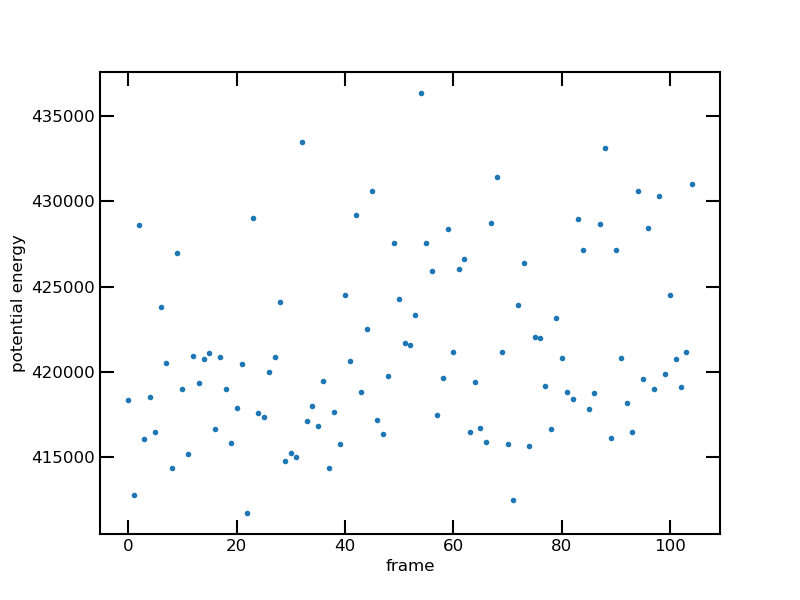
\includegraphics[width=\figwidth]{potential_energy_cell3_chrom1.png}
	\caption{Potential energy of all frames for simulation of chromosome 1 of cell 3 indiviually.}
	\label{fig:potential_energy_cell3_chrom1}
\end{figure}

Looking at the RMSD of the same chromsome simulation though, seen in Figure~\ref{fig:potential_energy_cell3_chrom1}, the mean RMSD relative to frame 22, which is the lowest potential energy frame, is quite high at \(\num{4.6(10)}\), suggesting this simulation does not reach a stable ground state. The mean RMSDs for chromosome 1 for all cells in Table~\ref{tab:chrom1_mean_rmsds} show that this is the case for all simulations of chromosome 1. Unsurprisingly, when comparing these individually simulated chromosomes with their respective counterparts in the simulation of the entire cell, by calculating the RMSD to the chromosome in the average trajectory, the results are similarly \textcolor{orange}{bad}. This implies that the structure of chromosome 1 when simulated individually is quite dissimilar to the structure when simulated in the context of the entire cell.

\begin{figure}[ht]
\centering
	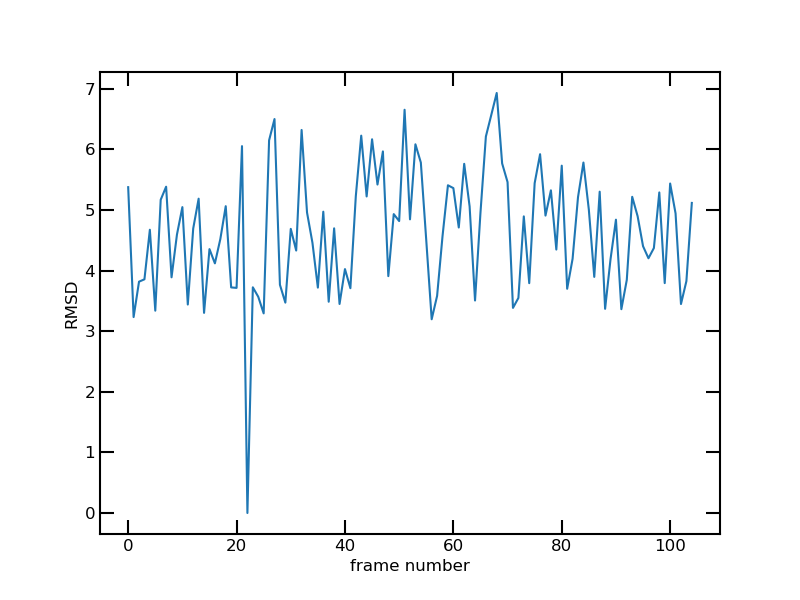
\includegraphics[width=\figwidth]{rmsd_cell3_chrom1.png}
	\caption{RMSD of each frame of the simulation of chromosome 1 of cell 3 with the lowest-energy frame, frame 22.}
	\label{fig:rmsd_cell3_chrom1}
\end{figure}

% section chromosome_1 (end)


\section{Chromosome 19} % (fold)
\label{sec:chromosome_19}

The same analysis has be repeated for chromosome 19, which is the shortest chromosome with only 584 beads compared to chromosome 1 with 1924 beads. The results can be seen in Table~\ref{tab:chrom19_mean_rmsds}. While most of the RMSDs are similarly high, especially for cell 1 and cell 4 the mean RMSD to the average simulated cell drops to \(2.3\) and \(1.5\) respectively, which is indicative of significant resemblance. Nevertheless, generally the difference between the individually simulated chromosomes and the chromosomes in the cell is quite high, implying the stabilising effect of other chromosomes is a non-neglegible factor for determining a chromosomes structure.

\begin{table}[ht]
\centering
  \caption{Mean of RMSDs between each frame of chrosomome 1 simulation to lowest energy frame of this simulation and to chromosome 1 in the average trajectory of the entire cell simulation for each cell.}
  \label{tab:chrom1_mean_rmsds}
  \sisetup{ table-alignment-mode=none }
  \begin{tabular}{l @{\phantom{abc}} S S S S S S S S}
  \toprule
    Cell & 1 & 2 & 3 & 4 & 5 & 6 & 7 & 8 \\
  \midrule
    \parbox{4cm}{Mean RMSD to \\ lowest energy frame} & 4.6 & 3.4 & 4.6 & 2.5 & 4.2 & 3.2 & 4.9 & 8.2 \\
    Mean RMSD to avg cell & 4.6 & 3.9 & 5.6 & 3.1 & 4.6 & 6.8 & 5.1 & 7.8 \\
  % \midrule
  %   Internal contacts & 3735 & 2594 & 1231 & 3197 & 2323 & 2860 & 1599 & 1310 \\
  %   External contacts & 1562 & 660 & 854 & 384 & 849 & 294 & 300 & 349 \\
  %   \parbox{4cm}{\centering Proportion of \\ internal contacts} & 71\% & 80\% & 59\% & 89\% & 73\% & 91\% & 84\% & 79\% \\
  \bottomrule
  \end{tabular}
\end{table}

\begin{table}[ht]
\centering
  \caption{Mean of RMSDs between each frame of chrosomome 19 simulation to lowest energy frame of this simulation and to chromosome 19 in the average trajectory of the entire cell simulation for each cell.}
  \label{tab:chrom19_mean_rmsds}
  \sisetup{ table-alignment-mode=none }
  \begin{tabular}{l @{\phantom{abc}} S S S S S S S S}
  \toprule
    Cell & 1 & 2 & 3 & 4 & 5 & 6 & 7 & 8 \\
  \midrule
    \parbox{4cm}{Mean RMSD to \\ lowest energy frame} & 1.8 & 3.7 & 4.9 & 1.2 & 3.6 & 2.5 & 4.6 & 5.9 \\
    Mean RMSD to avg cell & 2.3 & 4.1 & 6.0 & 1.5 & 4.4 & 3.1 & 4.8 & 6.1 \\
  % \midrule
  %   Internal contacts & 1229 & 717 & 243 & 1037 & 684 & 761 & 460 & 333 \\
  %   External contacts & 605 & 394 & 544 & 214 & 381 & 302 & 142 & 169 \\
  %   \parbox{4cm}{\centering Proportion of \\ internal contacts} & 67\% & 65\% & 31\% & 83\% & 64\% & 72\% & 76\% & 66\% \\
  \bottomrule
  \end{tabular}
\end{table}

% section chromosome_19 (end)

% One possible explanation for the dissimililarity betwen the chrosomosome structure in the cell and individually could be that the chromosome structure gets stabilised by its contacts with other chromosomes. To examine the strength of this effect the number of Hi-C contacts of the chromosome both with itself and and with other contacts and then calculate the ratio of internal contacts.

% chapter individual_chromosomes (end)